\documentclass[a4paper,titlepage,12pt]{scrbook}
\usepackage{header}

\RCSdef $Revision: 1.4 $
\RCSdef $Date: 2004/06/26 18:27:28 $

%\newcommand\version{Version \today \xspace}
\newcommand\version{Version 1.0\xspace}

\title {\huge \product\\[0.5cm]\large User Manual \\[0.5cm] \version
  \\[1cm] \Large \company}



\begin{document}

%%%%%%%%%%%%%%%%%%%%%%%%%%%%%%%%%%%%%%%%%%%%%%%%%%%%%%%%%%%%%%%%%%%%%%%%%%%%%%%
%% Deckblatt

\begin{titlepage}
\renewcommand{\thefootnote}{\fnsymbol{footnote}}
{\Huge
\raggedright
\textbf{\bf Kobold} \\
\huge Product Line Management System
\rule{\textwidth}{0.75pt}
\par
}
\begin{flushleft}
\normalsize
\version
\end{flushleft}


\vfill

\includegraphics[width=15cm]{../common/logo-color.png}
\vfill
{\parindent=0cm
\Huge User Manual
}


\setcounter{footnote}{0}
\end{titlepage}

%%%%%%%%%%%%%%%%%%%%%%%%%%%%%%%%%%%%%%%%%%%%%%%%%%%%%%%%%%%%%%%%%%%%%%%%%%%%%%%
%% Version history

\section*{Version history}

\begin{itemize}

\item Version 1.0 (2004-05-18)

\end{itemize}

%%%%%%%%%%%%%%%%%%%%%%%%%%%%%%%%%%%%%%%%%%%%%%%%%%%%%%%%%%%%%%%%%%%%%%%%%%%%%%%
%% Inhaltsverzeichnis
\tableofcontents


%%%%%%%%%%%%%%%%%%%%%%%%%%%%%%%%%%%%%%%%%%%%%%%%%%%%%%%%%%%%%%%%%%%%%%%%%%%%%%%%%%% 
\chapter{Introduction}

\section{About this document}

This manual provides instructions for the installation and usage of the
product line management system Kobold.

\section{The Kobold System}

The primary purpose of Kobold is to provide a tool for the development
and maintenance of software product lines. Kobold also supports the
establishment of a role-based development process.

\section{Structure of this document}
This user manual will help you to install the Kobold system and to
determine the technical conditions. \par
The description of the usage is divided in two parts. The first part
will introduce Kobold on the basis of some simple examples. This tutorial
will enable you to start working with Kobold right away. \par
The second part will provide detailed descriptions of each window and
each menu item. This will help you answer your questions while working
with Kobold.
\chapter{Technical Requirements}

Kobold runs on 

\begin{itemize}
\item Windows NT/2000/XP
\item Linux (Motif)
\item Linux (GTK 2)
\item Solaris 8 (SPARC/Motif)
\item QNX (x86/Photon)
\item AIX (PPC/Motif)
\item HP-UX (HP9000/Motif)
\item Mac OSX (Mac/Cocoa)
\end{itemize}

with the following requirements: \par

\begin{itemize}
\item 400 MHz
\item 256 MB main memory
\item 200 MB fixed-disk storage
\item Java 2 version 1.4
\item Eclipse 3.0
\end{itemize}
\par
\par

Its server is purely based on Java and therefore runs on:
\begin{itemize}
\item Solaris-SPARC
\item Windows NT/2000/XP
\item Linux
\end{itemize}

\chapter{Instructions for Installation}

\subsection{Checking out the files}
After you have started Eclipse 3.0, change to CVS Repositories perspective and add a CVS repository. \par
Enter the following data (see \ref{neuesrep}):
\begin{itemize}
\item host: cvs.berlios.de
\item repository path: /cvsroot/kobold
\item user: anonymous
\end{itemize}
Leave the remaining data untouched and confirm the dialog. \par

\begin{figure}[h!]
\begin{center}
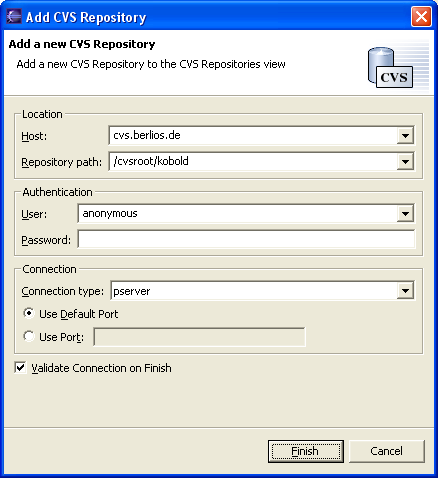
\includegraphics[width=12cm]{neuesrep.png}
   \caption{Adding a new repository}�
\label{neuesrep}
\end{center}
\end{figure}

Open the tree along HEAD, kobold and src (see \ref{auschecken}). Check out the four folders kobold.client.plam,
kobold.client.vcm, kobold.common and kobold.server through 'check out as..' (context menue)
and confirm with 'Finish'.

\begin{figure}[h!]
\begin{center}

\includegraphics[width=10cm]{auschecken.png}
   \caption{This is how your tree should look like}
\label{auschecken}
\end{center}
\end{figure}\par

Open the 'Window' menu and select 'preferences'. Select 'plug-in development' and 'Target 
Platform' and press the button 'Not in Workspace'. Confirm with OK. \par

Projects kobold.client.plam, kobold.client.vcm and kobold.common: \par
Right-click on the project and select 'properties'. Select 'Java build path' and the 'source'
tab. Remove the existing entry and add a new one by pressing 'Add Folder'. Choose the 
src-folder and confirm. Append '/bin' to the default output folder (see \ref{buildpath}).
 Close the preferences dialog. \par

\begin{figure}[h!]
\begin{center}
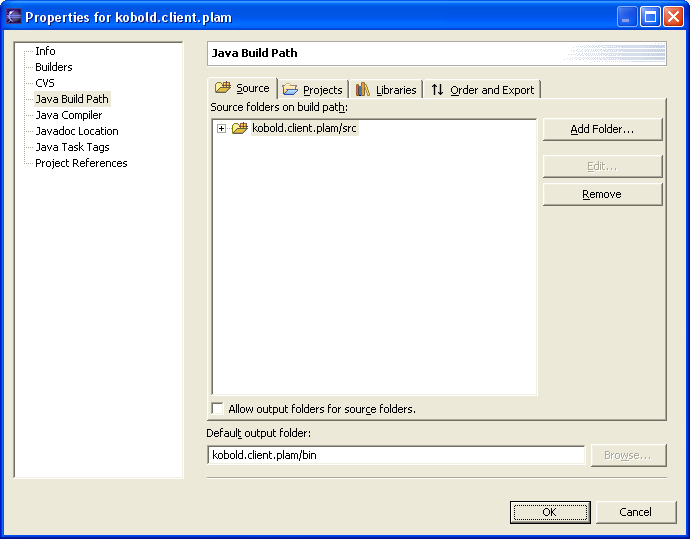
\includegraphics[width=15cm]{buildpath.png}
   \caption{This is how your buildpath should look like}
\label{buildpath}
\end{center}
\end{figure}\par

Projects kobold.server: \par
Right-click on the project and select 'properties'. Select 'Java build path' and the 'source'
tab. Remove the existing entry and add a new one by pressing 'Add Folder'. Choose the 
src-folder and confirm. Append '/bin' to the default output folder. 
Switch to the 'projects' tab and select 'kobold.common'. Close the preferences 
dialog. \par

Again, right-click on the project kobold.client.plam and select 'update classpath'. Select 
kobold.client.plam, kobold.client.vcm and kobold.common and confirm.

\subsection{Setting the correct properties}


First of all edit the server.properties
file from {\it kobold.server/server.properties} to suite your local
requirements. Under UNIX this file might look similiar to the following
bits:

\begin{verbatim}
# Note storePath is the prefix path for all kobold stores!
kobold.server.storePath=/tmp/
kobold.server.globalMessageStore=global.xml
kobold.server.messageStore=messages.xml
kobold.server.productStore=product.xml
kobold.server.userStore=user.xml
#
java.protocol.handler.pkgs=com.sun.net.ssl.internal.www.protocol
javax.net.debug=all
javax.net.ssl.keyStore=../kobold.common/scripts/keystore
javax.net.ssl.keyStorePassword=kobold1
javax.net.ssl.trustStore=../kobold.common/scripts/truststore
javax.net.ssl.trustStorePassword=kobold1
\end{verbatim}

Under Windows-based systems you've to change the paths into a
DOS-alike format.

In the following table all properties are described in detail:

\begin{tabular}{|l|l|l|}\hline
\textbf{Property} &  \textbf{Description}\\ \hline
kobold.server.storePath  & destination path for files stored by the server \\ \hline
kobold.server.globalMessageStore & file name to store global messages \\
    \hline
kobold.server.messageStore & file name to store pending messages \\
    \hline
kobold.server.productStore & file name to store products and
productlines \\ \hline
kobold.server.userStore & file name to store user data \\ \hline
java.protocol.handler.pkgs & default protocol to commincate \\ \hline
javax.net.debug & debug level of net communication \\ \hline
javax.net.ssl.keyStore & path to your SSL keystore \\ \hline
javax.net.ssl.keyStorePassword & password to access your SSL keystore \\
    \hline
javax.net.ssl.trustStore & path to your SSL truststore \\ \hline
javax.net.ssl.trustStorePassword & password to access your SSL
truststore \\ \hline
\end{tabular}

You also have to edit the sat.properties file from {\it kobold.client.serveradmin/sat.properties} 
to suite your local
requirements. Under UNIX this file might look similiar to the following
bits:

\begin{verbatim}
#used to communicate with Kobold servers via ssl
java.protocol.handler.pkgs=com.sun.net.ssl.internal.www.protocol
javax.net.debug=all
javax.net.ssl.keyStore=/home/garbeam/eclipse/kobold.common/scripts/keystore
javax.net.ssl.keyStorePassword=kobold1
javax.net.ssl.trustStore=/home/garbeam/eclipse/kobold.common/scripts/truststore
javax.net.ssl.trustStorePassword=kobold1
\end{verbatim}

As you can see, it contains the same properties as the {\it
server.properties} file for SSL communication, but since the Kobold
client is independent from the server it has it's own properties.\par

Right after your first start of the Kobold Client Feater Set, change the Kobold
preferences so that the client-server communication works properly. For more
information go to the tutorial section.
\chapter{The concepts in Kobold}

\section{Productline}

Kobold is a tool to administrate productlines. By specifying an architecture in which
core assets are linked with each other through dependency and exclusion edges, the product line engineer
creates a basis for all the products of the product line. 

\section{Component}

Components are abstract modules in the productline architecture. Instances of them (i.d. variants and custom components)
are used for the different products of the productline.

\section{Custom Component}

Custom components are instances of components and used in product architectures. They can
differ from the corresponding components in order to fit the product.

\section{Variant}

Variants are modifications of components.

\section{Release}

Releases are created to save the current state of a variant. 

\section{Meta Node}

Meta nodes are a means to creating complex relationships between nodes. They represent
the relationships AND and OR.

\section{Dependency Edge}

A dependency edge indicates that the nodes connected by the edge depend on each other.
Therefore one of them can't be used without the other.

\section{Exclusion Edge}

An exclusion edge indicates that the nodes connected by the edge can't be used
in the same product.

\section{GXL}

GXL is a graph exchange language and used to export the architecture, etc. For more
information: http://www.gupro.de/GXL/

\section{Product Line Engineer (PLE)}

The product line engineer has the responsibility for the product line.

\section{Product Engineer (PE)}

The product engineer administrates a specific product and is a subordinate of the
product line engineer.

\section{Product Developer (P)}

Product developers are subordinates of the product engineer. They develop the software 
product.

\section{Workflow}

A workflow is a working process. You can create them in order to trigger certain
activities when the server executes one of the following commands:

\begin{itemize}
	\item login
	\item logout
	\item get roles
	\item get product role
	\item add user
	\item get productline
	\item get product
	\item add product
	\item add role
	\item remove role
	\item apply productline modifications
	\item apply product modifications
	\item remove user
\end{itemize}
\chapter{Tutorial}

\section{Getting started}

\subsection{Kobold Server}

To start the Kobold server within Eclipse just select 'Run...' in the
'Run' menu from
Eclipse and select the class
{\it kobold.server.SecureKoboldWebServer} with a numerical programm argument for
the port it should listen for connections. 
You've to enter only one VM argument which is needed to locate the {\it
server.properties} file and to suite your local requirements: \par

\begin{verbatim}
-Dkobold.server.configFile=/home/garbeam/eclipse/
kobold.server/server.properties
\end{verbatim}

Make sure that your {\it \$CLASSPATH} environment contains all JARs
provided by\\
 {\it kobold.common/contrib} beside a Java2 JRE and the Sun
JSSE classes (included by Sun JDK 1.4).

\subsection{Kobold Client Feature Set}
To start the Kobold client feature set from within Eclipse (which is
currently the only way) just select 'Run...' in the 'Run' menu and
double-click 'Run-time Workbench'. A new configuration is created which you 
can name as you wish (see \ref{run}). 

\begin{figure}[h!]
\begin{center}
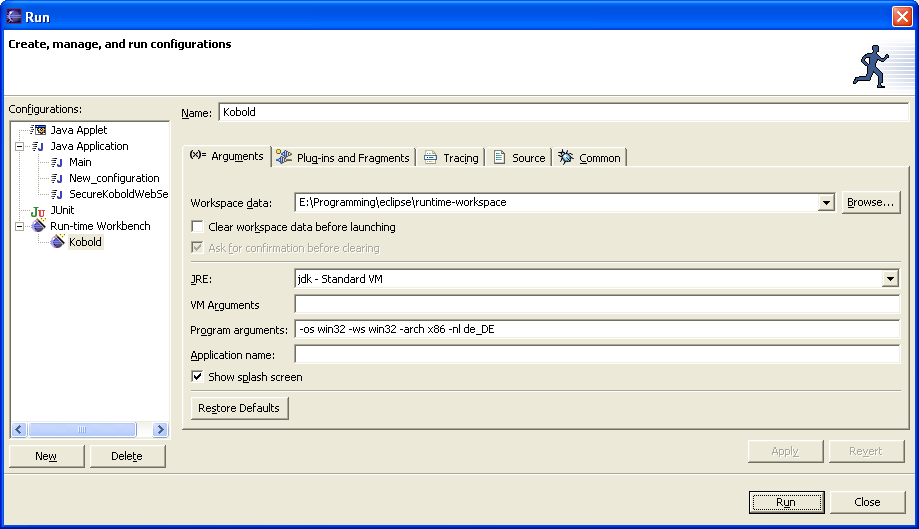
\includegraphics[width=15cm]{run.png}
   \caption{The Run dialog}
\label{run}
\end{center}
\end{figure}\par

Confirm with 'Run'.

A new Eclipse instance will open with the Kobold feature set enabled.


\subsection{Kobold Server Administration Tool}
To start the Kobold Server Administration Tool within Eclipse just select 'Run...' in the
'Run' menu from
Eclipse and select the class
{\it kobold.client.serveradmin.ServerAdministrationTool}.

You've to enter only one VM argument which is needed to locate the {\it
sat.properties} file and to suite your local requirements: \par

\begin{verbatim}
-Dkobold.sat.configFile=/home/garbeam/eclipse/
kobold.client.serveradmin/sat.properties
\end{verbatim}

\section{Setting the Kobold preferences}
In the Kobold Client menu, select 'Window' and then 'Preferences'. The preferences
dialog opens (see \ref{pref}). Select 'Kobold' and enter the properties for the Kobold Client.
They resemble your SAT properties (see chapter 'Installation').

\begin{figure}[h!]
\begin{center}
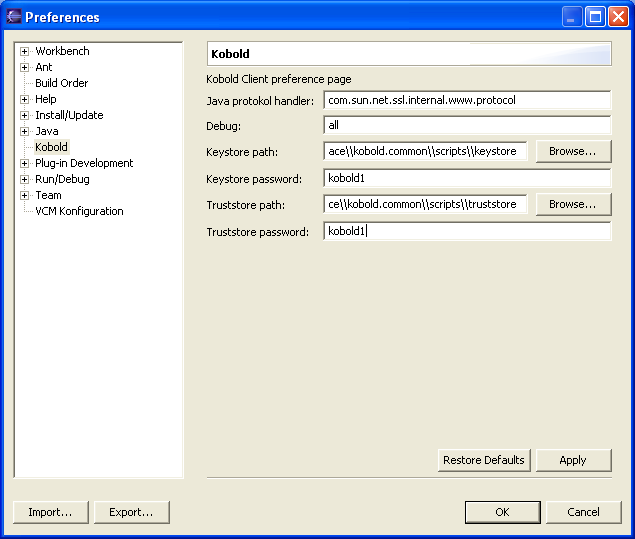
\includegraphics[width=10cm]{pref.png}
   \caption{Kobold preferences}
\label{pref}
\end{center}
\end{figure}\par

\section{Product-related}

\subsection{Checking out a product(line)}

In the File menu select 'New' and then 'Kobold PLAM Project'. The Kobold wizard opens.
Enter the url of your Kobold server, your username and password. Then press
"test connection". If the test succeeds, the "next" button is enabled (see \ref{wizard1}).

\begin{figure}[h!]
\begin{center}
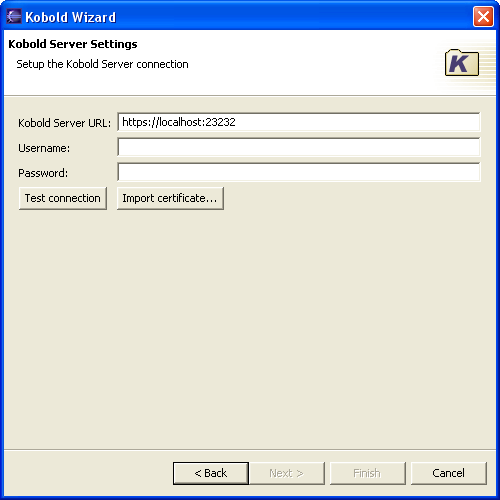
\includegraphics[width=10cm]{wizard1.png}
   \caption{Kobold wizard}
\label{wizard1}
\end{center}
\end{figure}\par

After that you choose the product(line) you want to check out (see \ref{wizard2}).

\begin{figure}[h!]
\begin{center}

\includegraphics[width=10cm]{wizard2.png}
   \caption{Kobold wizard}
\label{wizard2}
\end{center}
\end{figure}\par

In the last step you have to enter the name of the project you want to create (see \ref{wizard3}).

\begin{figure}[h!]
\begin{center}
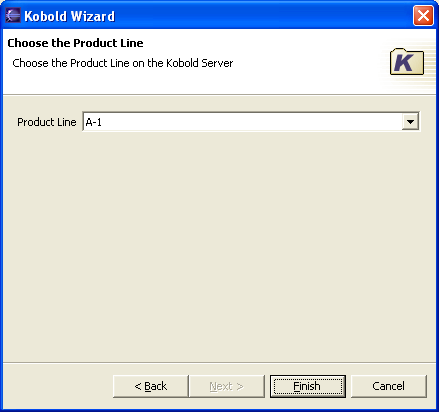
\includegraphics[width=10cm]{wizard3.png}
   \caption{Kobold wizard}
\label{wizard3}
\end{center}
\end{figure}\par

A new project has been created. You can open the different views through the Window menu
and 'show view'. 

\subsection{Creating a product}

In the palette press 'compose product'. The components, etc. in the architecture view turn
grey. You can now select the components, variants and releases you want to include into
you new product. The chosen objects turn blue (see \ref{compose}).

\begin{figure}[h!]
\begin{center}

\includegraphics[width=10cm]{composeproduct.png}
   \caption{Composing a Product}
\label{compose}
\end{center}
\end{figure}\par

%TODO: wie geht's weiter!

%\subsection{Renaming a product}

%Right-click on the product and choose "rename product" in the context menu. You can
%now enter a new name which will be used in the repository and the product line tree.

%TODO: Screenshot einf�gen

%\subsection{Changing a product}

%Right-click on the product and choose "change product". A wizard opens where you can
%change the CoreAssets for your product. 

%TODO: Screenshot einf�gen

%After you press "proceed", you are able
%to choose modules of other products from this product line. Press "Finish" and the changes
%are saved.

%\subsection{Setting a product on deprecated}

%Right-click on the product and choose "set on deprecated". Confirm your choice in
%the upcoming dialog and the product is deprecated. Its modules can no longer be
%used in a product.

%TODO: Screenshot einf�gen


\section{Node-related}

%\subsection{Creating a Core Asset}

%In the pallete select the "core asset" tool. Click into the Architecture Editor and
%a core asset is inserted. A dialog opens where you can enter the meta data of
%the core asset. Per drag+drop you can simply change the size of the core
%asset. \par
%Note: Core assets can only be inserted on the top-level plane of the Architecture Editor.

%TODO: Screenshot einf�gen


\subsection{Creating a component}

In the pallete select the "component" tool. Click and drag within a variant or top-level in 
the Architecture Editor. A component is inserted (see \ref{component}) and a dialog opens where you can enter the meta data of
the component. Per drag+drop you can simply change the size of the component. \par
Note: Components can only be inserted top-level or into variants.

\begin{figure}[h!]
\begin{center}

\includegraphics[width=8cm]{component.png}
   \caption{Component}
\label{component}
\end{center}
\end{figure}\par


\subsection{Creating a variant}

In the pallete select the "variant" tool. Click and drag within a component in 
the Architecture Editor. A variant is inserted (see \ref{variant}) and a dialog opens where you can enter the meta data of
the variant. Per drag+drop you can simply change the size of the variant. \par
Note: Variants can only be inserted into components.

\begin{figure}[h!]
\begin{center}

\includegraphics[width=10cm]{variant.png}
   \caption{Variant}
\label{variant}
\end{center}
\end{figure}\par


\subsection{Creating a release}

In the pallete select the "release" tool. Click and drag within a variant in 
the Architecture Editor. A release is inserted (see \ref{release}) and a dialog opens where you can enter the meta data of
the release. For each file of the variant you can select the revision number you want to add to the release. 
Per drag+drop you can simply change the size of the release. \par
Note: Releases can only be inserted into variants.

\begin{figure}[h!]
\begin{center}

\includegraphics[width=10cm]{release.png}
   \caption{Release}
\label{release}
\end{center}
\end{figure}\par

\subsection{Creating a meta node}

In the pallete select the "meta node" tool. Click and drag within the Architecture Editor. 
A meta node is inserted (see \ref{meta}). Possible meta node types are AND and OR. Be careful with
the direction of the edges that are linked to a meta node! In the following architecture component A
needs components B and C. But components B and C are independent of component A (see \ref{example}).

\begin{figure}[h!]
\begin{center}

\includegraphics[width=4cm]{metanode.png}
   \caption{Some meta nodes}
\label{meta}
\end{center}
\end{figure}\par

\begin{figure}[h!]
\begin{center}

\includegraphics[width=10cm]{example.png}
   \caption{Meta node example}
\label{example}
\end{center}
\end{figure}\par

\subsection{Deleting a component, variant or release}

Right-click on the item you want to delete and choose "delete" in the context
menu. Alternatively you
can select the item and press "Del" on your keyboard. Is the item used in other projects
you will be notified and be able to cancel the deletion process.

\subsection{Deleting a meta node}

Right-click on the meta node you want to delete and choose "delete" in the context
menu. Alternatively you
can select the node and press "Del" on your keyboard.

\subsection{Marking a component, variant or release as "deprecated"}
Right-click on the object and choose "configure". The Asset Configuration dialog (see \ref{config} and \ref{config2}) opens where you can
mark the check-box 'deprecated'. This sets the object on deprecated. Deprecated objects are grey with a 
red cross in the upper right-hand corner (see \ref{deprecated}).

\begin{figure}[h!]
\begin{center}
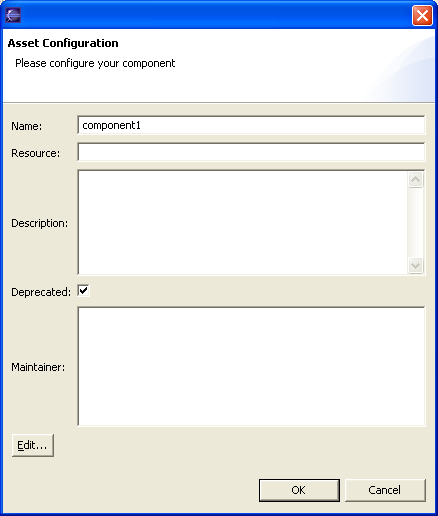
\includegraphics[width=10cm]{config.png}
   \caption{Asset Configuration dialog (component)}
\label{config}
\end{center}
\end{figure}\par

\begin{figure}[h!]
\begin{center}

\includegraphics[width=7cm]{deprecated.png}
   \caption{Deprecated component}
\label{deprecated}
\end{center}
\end{figure}\par

\subsection{Setting the maintainers of a component}
Right-click on the component and choose "configure". The Asset Configuration dialog (see \ref{config}) opens.
Press the 'Edit...' button. A new window opens where you can select the users you want to make maintainers of
the component (see \ref{maintainer}). After pressing 'OK' you can see the new maintainers in the Asset Configuration
dialog.

\begin{figure}[h!]
\begin{center}
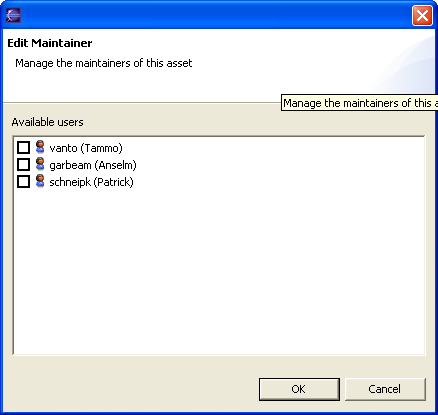
\includegraphics[width=10cm]{maintainer.png}
   \caption{Selecting maintainers}
\label{maintainer}
\end{center}
\end{figure}\par

\subsection{Selecting resources for a release}
Right-click on the component and choose "configure". The Asset Configuration dialog (see \ref{config2}) opens.
In the bottom of the dialog you can select the files of the variant you want to include into the release.

\begin{figure}[h!]
\begin{center}
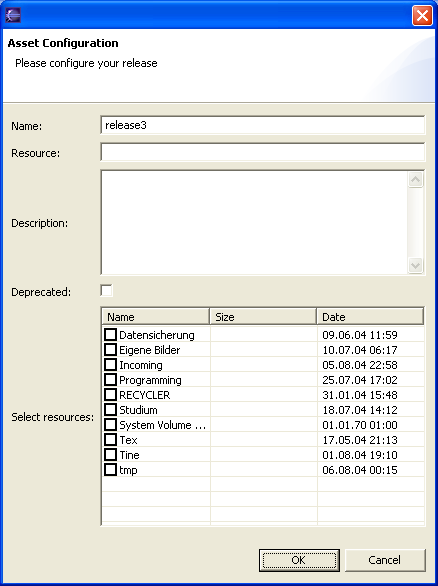
\includegraphics[width=10cm]{config2.png}
   \caption{Asset Configuration dialog (release)}
\label{config2}
\end{center}
\end{figure}\par

\subsection{Moving an item}
You can move any item per drag+drop.

\subsection{Changing the size of an item}
You can change the size of an item per drag+drop.

%\subsection{Creating a custom component}

%In the pallete select the "custom component" tool. Click into the Architecture 
%Editor. A component is inserted. A dialog opens where you can enter the meta data of
%the component. Per drag+drop you can simply change the size of the component. \par

%TODO: Screenshot einf�gen

%\subsection{Deleting a custom component}

%Right-click on the component you want to delete and choose "delete" in the context
%menu. Alternatively you
%can select the component and press "Del" on your keyboard. 


%\subsection{Setting a module on deprecated}

%Right-click on the module and choose "set on deprecated". Confirm your choice in
%the upcoming dialog and the module is deprecated. It can no longer be
%used in a product.

%TODO: Screenshot einf�gen



\section{Edge-related}

\subsection{Creating a dependency edge}

In the pallete select the "include edge" tool. Select an item in the Architecture Editor
as the starting point. The next item you select will be the aiming point (see \ref{include}).

\begin{figure}[h!]
\begin{center}

\includegraphics[width=10cm]{include.png}
   \caption{Dependency edge}
\label{include}
\end{center}
\end{figure}\par

\subsection{Creating an exclusion edge}

In the pallete select the "exclude edge" tool. Select an item in the Architecture Editor
as the starting point. The next item you select will be the aiming point (see \ref{exclude}).

\begin{figure}[h!]
\begin{center}

\includegraphics[width=10cm]{exclude.png}
   \caption{Exclusion edge}
\label{exclude}
\end{center}
\end{figure}\par

\subsection{Deleting an edge}

Right-click on the edge you want to delete and choose "delete" in the context menu.
Alternatively you can select the edge and press "Del" on your keyboard.


\section{Message-related}

\subsection{Writing a mail}

In the menu of the Workflow View select "new mail". A Workflow window opens where
you can enter your message, the subject and the recipient of the message. Send the
message by pressing the "Send" button. Pressing the "Cancel" button will close the window
without sending your message (see \ref{writemail}).

\begin{figure}[h!]
\begin{center}
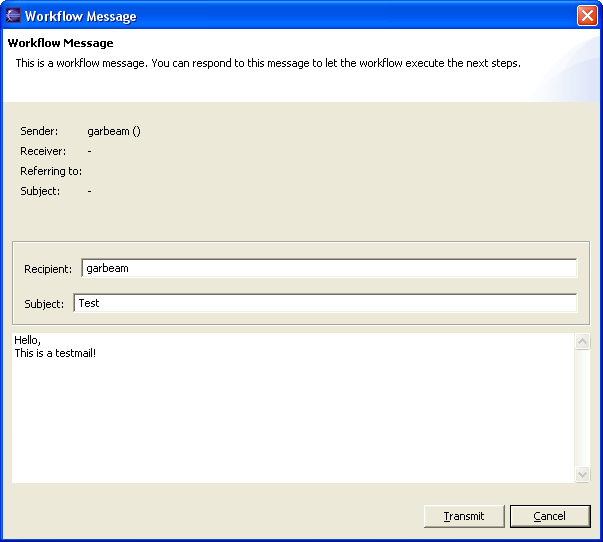
\includegraphics[width=10cm]{writemail.png}
   \caption{Write a new mail}
\label{writemail}
\end{center}
\end{figure}\par

\subsection{Answering a mail}

In the Workflow View double-click on the mail you want to answer. A Workflow
window opens where you can see the message text of the mail. Below you can enter
the subject and the text of your reply. Send the answer by pressing the "Send" 
button. Pressing the "Cancel" button will close the window without sending 
your message (see \ref{answermail}).

\begin{figure}[h!]
\begin{center}
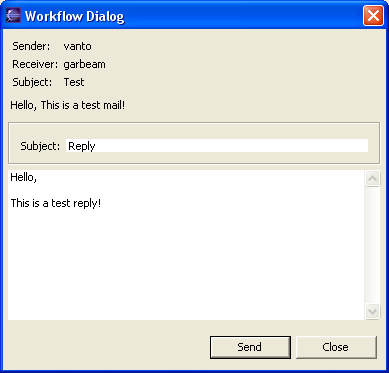
\includegraphics[width=10cm]{answermail.png}
   \caption{Answer a mail}
\label{answermail}
\end{center}
\end{figure}\par

\subsection{Deleting a message}

Right-click on the message and choose "Delete message" in the context menu.

\subsection {Fetching messages}

Select a project. Right-click in the Workflow View or open the corresponding menu. Choose "Fetch message".
Your new messages are being fetched and displayed in the Workflow View.

%\subsection {Filtering the Workflow View}

%(still undefined)

\subsection{Suggesting a file for a Core Group}

Note: This option should only be used by programmers!\par
In the menu of the Workflow View select "Suggest file for core group". A Workflow
window opens where you can enter the name of the file, its path and the username of the
PE you want to send the message to. You can also enter an additional comment you want 
the PE to read. Send the message by pressing the "Send" 
button. Pressing the "Cancel" button will close the window without sending 
your message (see \ref{core1}).

\begin{figure}[h!]
\begin{center}
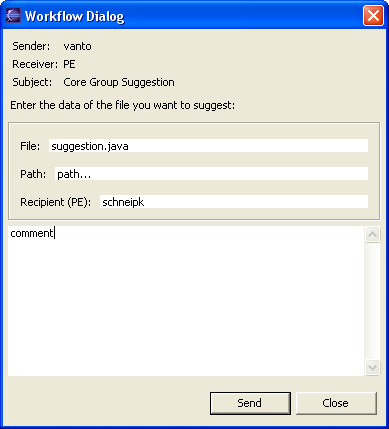
\includegraphics[width=10cm]{core1.png}
   \caption{Suggesting a file for a Core Group}
\label{core1}
\end{center}
\end{figure}\par

\subsection{Dealing with a Core Group suggestion}

In the Workflow View double-click on the Core Group suggestion message. A Workflow
window opens where you can see the message of the programmer (see \ref{core2}) or PE (see \ref{core3}). Below you
can select whether you agree to the suggestion or whether you decline it. You can also
enter an additional comment if you like. Send the message by pressing the "Send" 
button. Pressing the "Cancel" button will close the window without sending 
your message.\par
Note: The file will not be automatically uploaded and committed. The PLE has to do
this manually.

\begin{figure}[h!]
\begin{center}
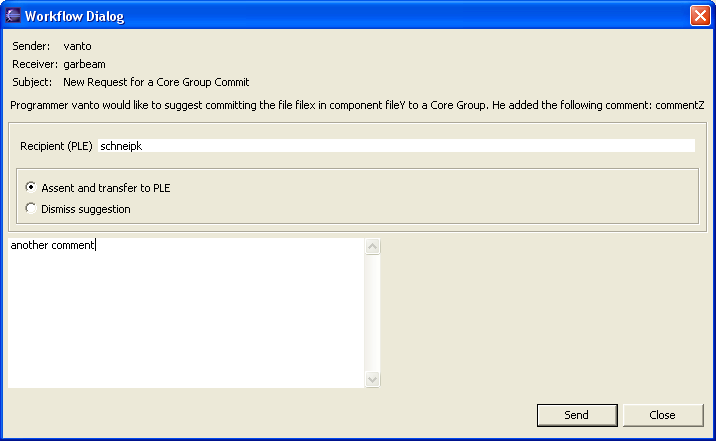
\includegraphics[width=10cm]{core2.png}
   \caption{Dealing with a Core Group suggestion - PE}
\label{core2}
\end{center}
\end{figure}\par

\begin{figure}[h!]
\begin{center}
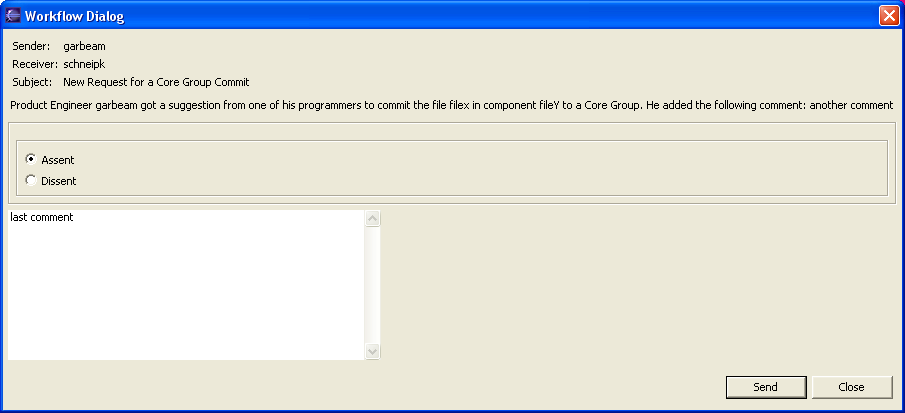
\includegraphics[width=10cm]{core3.png}
   \caption{Dealing with a Core Group suggestion - PLE}
\label{core3}
\end{center}
\end{figure}\par

\section{Exporting through GXL}

Select the productline, product, component or variant you want to export. In the
context menu of the object select "export" (see \ref{archcontext}). A wizard opens (see \ref{export}) where you can choose
whether to create a jar-file of the selected source or not. You should then enter
the path and names of the gxl-file and the jar-file. Alternatively you can enter 
the data through the "browse" dialog. To start the export, press the OK button.
You are able to see the status of your export in the wizard which will close after
the export is finished. If you decide not to do the export, simply press the 
"cancel" button.

\begin{figure}[h!]
\begin{center}

\includegraphics[width=10cm]{architecturekontext.png}
   \caption{Context menu of the Architecture View}
\label{archcontext}
\end{center}
\end{figure}\par

\begin{figure}[h!]
\begin{center}
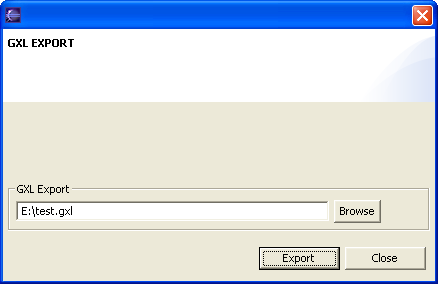
\includegraphics[width=10cm]{export.png}
   \caption{Export wizard}
\label{export}
\end{center}
\end{figure}\par


\section{Creating a Workflow}

Workflows are triggered by specific rules which you can find in the ruleset.drl file.
Here you can find some existing rules as an example. \par

A rule consists of the following parts:
\begin{itemize}
	\item name
	\item parameters
	\item conditions
	\item one consequence
\end{itemize}
Rules are a mixture of XML and Java.\par

This is what a sample rule looks like: \\

$<$rule name = "Name of the rule"$>$\\
\begin{quote}
$<$parameter identifier = "spy"$>$\\
\begin{quote}
$<$java:class$>$ kobold.common.data.RPCSpy $<$/java:class$>$\\
\end{quote}
$<$/parameter$>$\par
$<$java:condition$>$ spy.getMethodName().equals("login") $<$/java:condition$>$\par
$<$java:consequence$>$ System.out.println("Rule fired."); $<$/java:consequence$>$\\
\end{quote}
$<$/rule$>$\par


The rule will only be fired when its conditions are true. If there are several conditions,
all of the have to be true. Conditions and consequence are written in Java.\par

For your own rules, the rule's parameter will always be an RPCSpy object of the package
kobold.common.data. Such an object is created whenever an action is being executed by the server.
These are in detail (using their actual method names):
\begin{itemize}
	\item login
	\item logout
	\item addUser
	\item getAllUsers
	\item removeUser
	\item updateUserPassword
	\item updateUserFullName
	\item getProductlineNames
	\item getProductline
	\item updateProductline
	\item updateProduct
	\item updateComponent
\end{itemize}
The parameter RPCSpy will contain the methodName which you can get with the "getMethodName()" method. 
This returns one of the above Strings. An RPCSpy object also contains a vector of
arguments that were transmitted to the server for the execution. You have access to this vector through
the "getArguments()" method. \par
The ruleset.drl file contains a sample rule for adding a user. Whenever a new user is added, every other user
is notified. \par
In the last chapter you find the source code of the classes you need to work with for writing your own rules.
In order to have an up-to-date appendix, check out the complete Kobold module. 
Then enter the following command in the console within the directory of the user manual:

\begin{verbatim}
perl appendix.pl >appendix.tex
\end{verbatim}

After that, rebuild the usermanual.pdf.

%\section{Filtering the Architecture View}

%The toolbar of the Architecture Editor provides you with the following filterings:
%\begin{itemize}
%	\item Show/hide dependency edges
%	\item Show/hide exclusion edges
%	\item Show/hide synthetical edges
%	\item Show/hide deprecated components
%\end{itemize}

%TODO: Screenshot einf�gen

\section{Generating a metainfo document}
In the role tree right-click on the object (product line, component, variant, release) you want the metainfo document about
and select 'generate document...'. A 'Save as' dialog opens where you can select the parent folder into which the pdf-file
will be saved (see \ref{generate}). Confirm by pressing the 'OK' button and the pdf-file is created.

\begin{figure}[h!]
\begin{center}
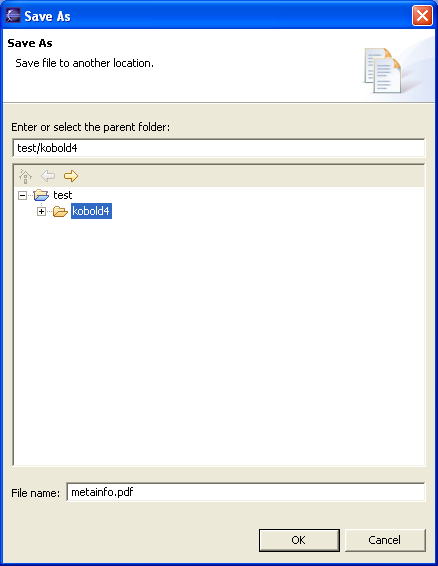
\includegraphics[width=10cm]{generate.png}
   \caption{Generate a metainfo document}
\label{generate}
\end{center}
\end{figure}\par

\section{Configuring an asset}
In the role tree right-click on the object (product line, component, variant, release) you want to configure
and select 'configure asset...'. The corresponding 'Asset Configuration' dialog opens where you can make your
changes (see \ref{config} and \ref{config2}).


\section{User-related}

\subsection{Creating a user}

Right-click in the role tree. In the context menu choose
'create new user'. The User Manager (see \ref{createuser1}) opens where you see a list of all existing users.
Push the 'create new user' button. In the opening dialog you can enter the username, real name and the
initial password of the user (see \ref{createuser2}). Pressing the 'OK' button creates the new user and you
can see the new user in the list of the User Manager.

\begin{figure}[h!]
\begin{center}
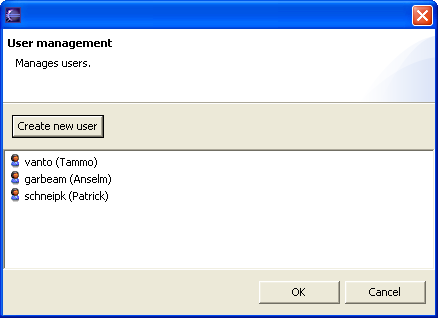
\includegraphics[width=10cm]{createuser1.png}
   \caption{Create a new user}
\label{createuser1}
\end{center}
\end{figure}\par

\begin{figure}[h!]
\begin{center}
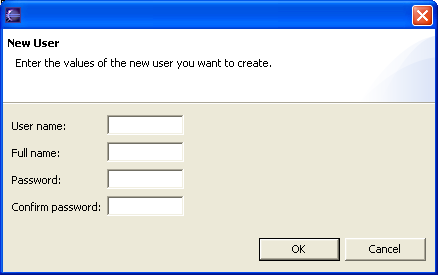
\includegraphics[width=10cm]{createuser2.png}
   \caption{Create a new user}
\label{createuser2}
\end{center}
\end{figure}\par

%\subsection{Changing a user role}

%Right-click on the corresponding product and choose "change role". A wizard opens.
%On the left side you can see a list of all existing users. On 
%the right side you can see lists of the product engineers and programmers that
%belong to the product. You can switch users from left to right and back by selecting
%the user and using
%the "<<" and ">>" buttons between the lists. In order to find a specific user in
%the left-hand list, enter the initial letters of the user. The list will then show
%only those usernames that start with the same letters. Press "Ok" when you are done
%and your changes are saved.

%TODO: Screenshot einf�gen

\subsection{Deleting a user}

Right-click in the role tree and select 'remove user'. A dialog opens with a list of all 
existing users (see \ref{delete}). Simply select the check-box next to the user you want to delete and confirm
with 'OK'. The user has been deleted.

\begin{figure}[h!]
\begin{center}
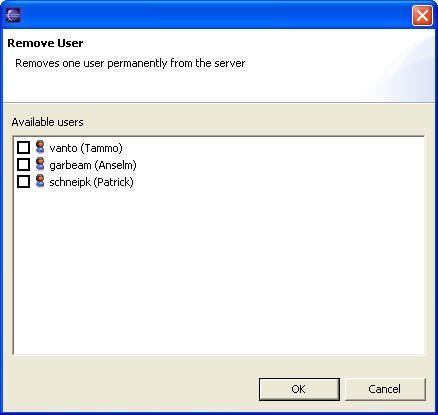
\includegraphics[width=10cm]{delete.png}
   \caption{Remove a user}
\label{delete}
\end{center}
\end{figure}\par

\subsection{Changing ones password}

Right-click in the role tree and select 'change password'. A dialog opens where you can
enter your new password (see \ref{password}). Confirm the password and press 'OK'. Your password has been changed.

\begin{figure}[h!]
\begin{center}
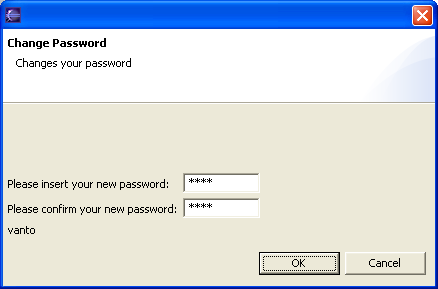
\includegraphics[width=10cm]{password.png}
   \caption{Change your password}
\label{password}
\end{center}
\end{figure}\par


\section{SAT-related}

\subsection{Creating a product line}
Enter the command "createpl". You are asked to enter the name of the new product
line and its meta data. Once you confirmed your entry, the product line is created.

\subsection{Deleting a product line}
Enter the command "removepl". You are then asked to enter the name of the product
line you want to remove. Once you confirmed your entry, the product line is deleted.

\subsection{Upgrading an existing user to PLE status}
Enter the command "addple". You are asked to enter the name of the person you want
to upgrade as PLE. Finally, enter the name of the product line you want to assign
the new PLE to. Once you confirmed your entry, the user has PLE rights.

\subsection{Removing PLE rights}
Enter the command "removeple". You are asked to enter the name of the user who shall 
no longer have PLE rights. Also, enter the name of the product line you want to
remove the PLE from. Once you confirmed your entry, the user is no longer PLE of
the entered product line.

\subsection{Getting a list of all existing commands}
Enter the command "help" and you get a list of all the commands of this tool and
their meanings.

\subsection{Exiting the tool}
Enter the command "exit".
\chapter{User Interface}

\section{Client}

The Kobold Client is based on Eclipse. Eclipse is a kind of universal tool 
platform - an open extensible IDE for anything and nothing in particular. Its 
user interface consists of views and editors. In editors you can both see and 
alter the data which is displayed whereas in views you can only look at the data 
but not alter it.

\subsection{Main Window}
In the Main Window you can see the following editors and views (see \ref{main}):
\begin{itemize}
	\item Architecture Editor
	\item Architecture Tree
	\item Workflow View
	\item Minimap
\end{itemize}

\begin{figure}[h!]
\begin{center}
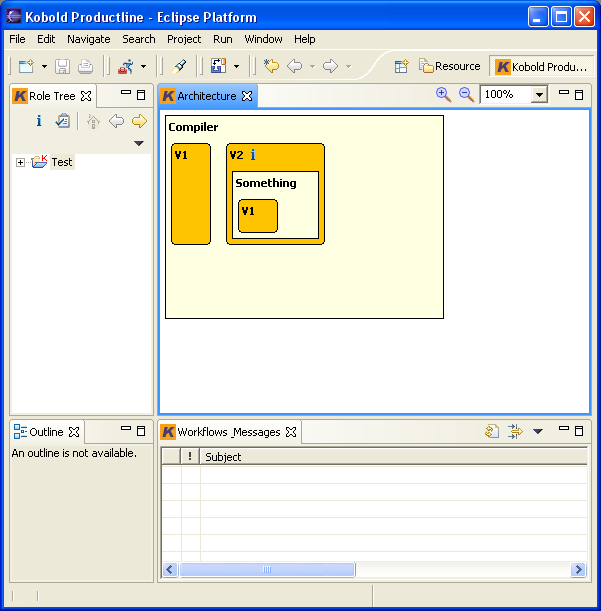
\includegraphics[width=15cm]{main.png}
   \caption{Main Window}
\label{main}
\end{center}
\end{figure}\par

The menu offers you in addition to the Eclipse standard options the following
possibilities:
\begin{itemize}
	\item Creating a new Kobold project
	\item Changing Kobold properties
\end{itemize}

\subsubsection{Creating a new project}

In the File menu select 'New' and then 'Kobold PLAM Project'. The Kobold wizard opens.
Enter the url of your Kobold server, your username and password. Then press
"test connection". If the test succeeds, the "next" button is enabled (see \ref{wizard1}).

\begin{figure}[h!]
\begin{center}
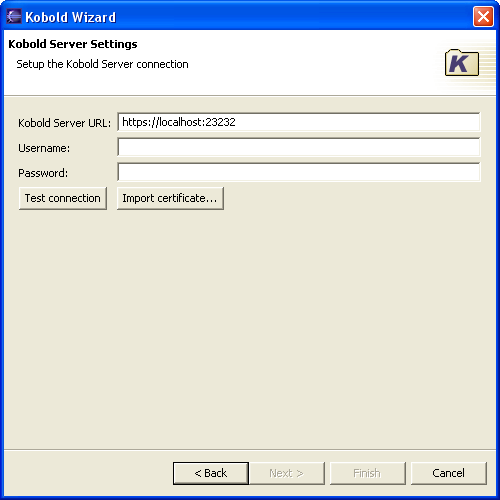
\includegraphics[width=10cm]{wizard1.png}
   \caption{Kobold wizard}
\label{wizard1}
\end{center}
\end{figure}\par

After that you choose the product(line) you want to check out (see \ref{wizard2}).

\begin{figure}[h!]
\begin{center}

\includegraphics[width=10cm]{wizard2.png}
   \caption{Kobold wizard}
\label{wizard2}
\end{center}
\end{figure}\par

In the last step you have to enter the name of the project you want to create (see \ref{wizard3}).

\begin{figure}[h!]
\begin{center}
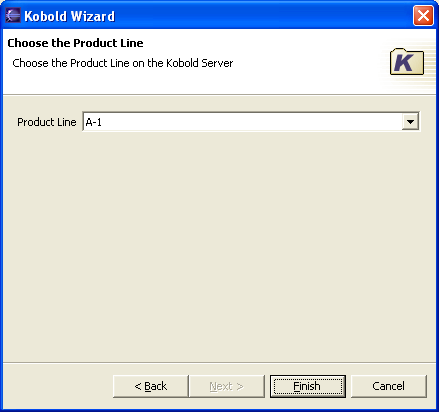
\includegraphics[width=10cm]{wizard3.png}
   \caption{Kobold wizard}
\label{wizard3}
\end{center}
\end{figure}\par

A new project has been created. You can open the different views and editors through the Window menu
and 'show view'. 

\subsubsection{Setting the Kobold preferences}
In the Kobold Client menu, select 'Window' and then 'Preferences'. The preferences
dialog opens (see \ref{pref}). Open the Kobold tree. In the SSL tab you can enter the 
properties for the Kobold Client. They resemble your SAT properties (see chapter 'Installation').
The VCM Configuration allows you to save your username, password and script for the
communication with the projects' repositories.

\begin{figure}[h!]
\begin{center}
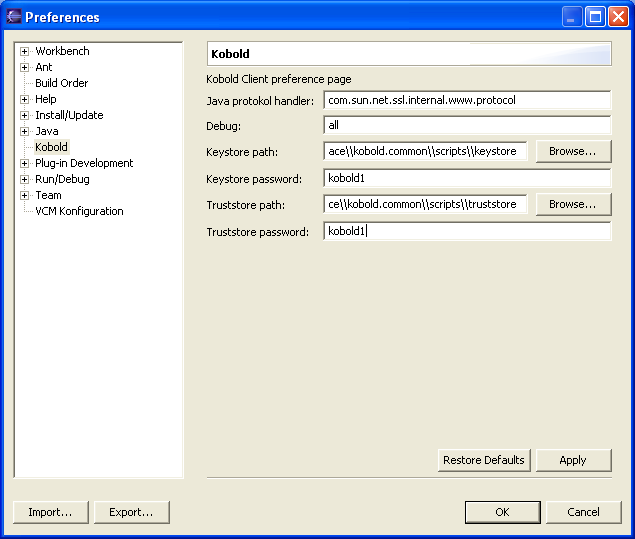
\includegraphics[width=14cm]{pref.png}
   \caption{Kobold preferences}
\label{pref}
\end{center}
\end{figure}\par



\subsection{Architecture Editor}

The Architecture Editor (see \ref{architecture}) displays the architecture of the product,
or productline respectively, that is selected in the Architecture Tree. \par

\begin{figure}[h!]
\begin{center}

\includegraphics[width=15cm]{architecture.png}
   \caption{Architecture Editor}
\label{architecture}
\end{center}
\end{figure}\par

Architectures are directed graphs that consist of nodes and edges. 
Nodes represent components, variants and releases. Directed edges represent
any relationship between nodes.\par

The Architecture Editor offers you the following options:
\begin{itemize}
	\item Creating a core asset/component
	\item Configuring a core asset/component
	\item Creating a variant
	\item Configuring a variant
	\item Creating a release
	\item Configuring a release
	\item Deleting a core asset/component, variant or release
	\item Creating a meta node
	\item Deleting a meta node
	\item Creating a dependency edge
	\item Creating an exclusion edge
	\item Deleting an edge
	\item Marking a component, variant or release "deprecated"
	\item Setting the maintainers of a component
	\item Moving an item
	\item Changing the size of an item
	\item Composing a product
	\item Export
\end{itemize}

Most of the options can be reached through the palette (see \ref{palette}).
You can find it to the right of the Architecture Editor. If offers you the tools
to work with the Architecture Editor and opens up when you click on it.

\begin{figure}[h!]
\begin{center}

\includegraphics[width=4cm]{palette.png}
   \caption{The palette}
\label{palette}
\end{center}
\end{figure}\par


\subsubsection{Creating a Core Asset/component}

In the pallete select the "component" tool. Click within a variant or top-level in 
the Architecture Editor. A component is inserted (see \ref{component}) and a dialog opens where you can enter the meta data of
the component. Per drag+drop you can simply change the size of the component. \par
Note: Core Assets/Components can only be inserted top-level or into variants.

\begin{figure}[h!]
\begin{center}

\includegraphics[width=8cm]{component.png}
   \caption{Component}
\label{component}
\end{center}
\end{figure}\par

\subsubsection{Configuring a core asset/component}


\subsubsection{Creating a variant}

In the pallete select the "variant" tool. Click within a component in 
the Architecture Editor. A variant is inserted (see \ref{variant}) and a dialog opens where you can enter the meta data of
the variant. Per drag+drop you can simply change the size of the variant. \par
Note: Variants can only be inserted into components.

\begin{figure}[h!]
\begin{center}

\includegraphics[width=10cm]{variant.png}
   \caption{Variant}
\label{variant}
\end{center}
\end{figure}\par


\subsubsection{Configuring a variant}


\subsubsection{Creating a release}

In the pallete select the "release" tool. Click within a variant in 
the Architecture Editor. A release is inserted (see \ref{release}) and a dialog opens where you can enter the meta data of
the release. For each file of the variant you can select the revision number you want to add to the release. 
Per drag+drop you can simply change the size of the release. \par
Note: Releases can only be inserted into variants.

\begin{figure}[h!]
\begin{center}

\includegraphics[width=10cm]{release.png}
   \caption{Release}
\label{release}
\end{center}
\end{figure}\par


\subsubsection{Configuring a release}
Right-click on the component and choose "configure". The Asset Configuration dialog (see \ref{config2}) opens.


\begin{figure}[h!]
\begin{center}
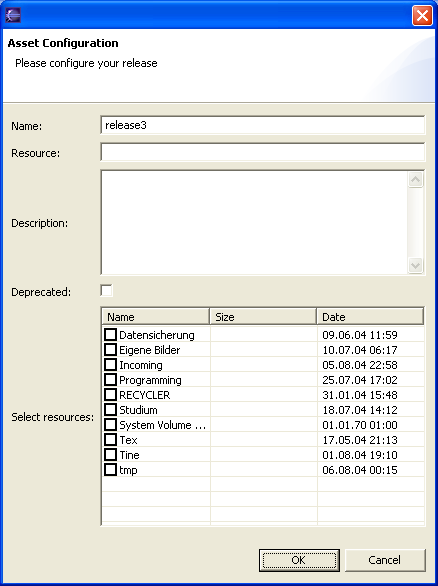
\includegraphics[width=10cm]{config2.png}
   \caption{Asset Configuration dialog (release)}
\label{config2}
\end{center}
\end{figure}\par


\subsubsection{Deleting a core asset/component, variant or release}

Right-click on the item you want to delete and choose "delete" in the context
menu. Alternatively you
can select the item and press "Del" on your keyboard. Is the item used in other projects
you will be notified and be able to cancel the deletion process.


\subsubsection{Creating a meta node}

In the pallete select the "meta node" tool. Click within the Architecture Editor. 
A meta node is inserted (see \ref{meta}). Possible meta node types are AND and OR. Be careful with
the direction of the edges that are linked to a meta node! In the following architecture component A
needs components B and C. But components B and C are independent of component A (see \ref{example}).

\begin{figure}[h!]
\begin{center}

\includegraphics[width=4cm]{metanode.png}
   \caption{Some meta nodes}
\label{meta}
\end{center}
\end{figure}\par

\begin{figure}[h!]
\begin{center}

\includegraphics[width=10cm]{example.png}
   \caption{Meta node example}
\label{example}
\end{center}
\end{figure}\par

\subsubsection{Deleting a meta node}

Right-click on the meta node you want to delete and choose "delete" in the context
menu. Alternatively you
can select the node and press "Del" on your keyboard.

\subsubsection{Marking a component, variant or release as "deprecated"}
Right-click on the object and choose "configure". The Asset Configuration dialog (see \ref{config} and \ref{config2}) opens where you can
mark the check-box 'deprecated'. This sets the object on deprecated. Deprecated objects are grey with a 
red cross in the upper right-hand corner (see \ref{deprecated}).

\begin{figure}[h!]
\begin{center}
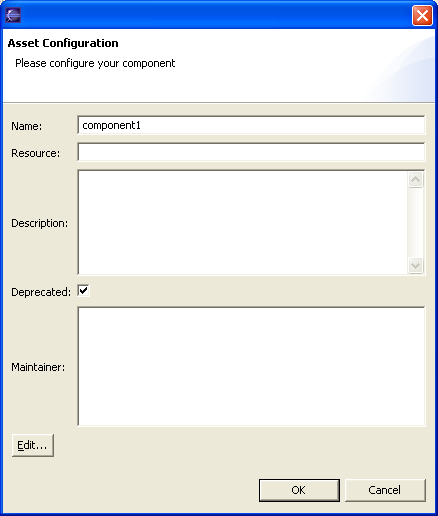
\includegraphics[width=10cm]{config.png}
   \caption{Asset Configuration dialog (component)}
\label{config}
\end{center}
\end{figure}\par

\begin{figure}[h!]
\begin{center}

\includegraphics[width=7cm]{deprecated.png}
   \caption{Deprecated component}
\label{deprecated}
\end{center}
\end{figure}\par



\subsubsection{Creating a dependency edge}

In the pallete select the "include edge" tool. Select an item in the Architecture Editor
as the starting point. The next item you select will be the aiming point (see \ref{include}).

\begin{figure}[h!]
\begin{center}

\includegraphics[width=10cm]{include.png}
   \caption{Dependency edge}
\label{include}
\end{center}
\end{figure}\par

\subsubsection{Creating an exclusion edge}

In the pallete select the "exclude edge" tool. Select an item in the Architecture Editor
as the starting point. The next item you select will be the aiming point (see \ref{exclude}).

\begin{figure}[h!]
\begin{center}

\includegraphics[width=10cm]{exclude.png}
   \caption{Exclusion edge}
\label{exclude}
\end{center}
\end{figure}\par

\subsubsection{Deleting an edge}

Right-click on the edge you want to delete and choose "delete" in the context menu.
Alternatively you can select the edge and press "Del" on your keyboard.


\subsubsection{Marking a component, variant or release as "deprecated"}
Right-click on the object and choose "configure". The Asset Configuration dialog (see \ref{config} and \ref{config2}) opens where you can
mark the check-box 'deprecated'. This sets the object on deprecated. Deprecated objects are grey with a 
red cross in the upper right-hand corner (see \ref{deprecated}).

\begin{figure}[h!]
\begin{center}
\includegraphics[width=10cm]{config.png}
   \caption{Asset Configuration dialog (component)}
\label{config}
\end{center}
\end{figure}\par

\begin{figure}[h!]
\begin{center}
\includegraphics[width=7cm]{deprecated.png}
   \caption{Deprecated component}
\label{deprecated}
\end{center}
\end{figure}\par


\subsubsection{Setting the maintainers of a component}
Right-click on the component and choose "configure". The Asset Configuration dialog (see \ref{config}) opens.
Press the 'Edit...' button. A new window opens where you can select the users you want to make maintainers of
the component (see \ref{maintainer}). After pressing 'OK' you can see the new maintainers in the Asset Configuration
dialog.

\begin{figure}[h!]
\begin{center}
\includegraphics[width=10cm]{maintainer.png}
   \caption{Selecting maintainers}
\label{maintainer}
\end{center}
\end{figure}\par


\subsubsection{Moving an item}
You can move any item per drag+drop.

\subsubsection{Changing the size of an item}
You can change the size of an item per drag+drop.


\subsubsection{Composing a product}

In the palette press 'compose product'. The components, etc. in the architecture view turn
grey. You can now select the components, variants and releases you want to include into
you new product. The chosen objects turn blue (see \ref{compose}). When done press the 
'create product' button in the Architecture Editor. A dialog opens where you can enter
the name and metainfo of your new product. After confirming the dialog, you can see
your new product in the Role View.

\begin{figure}[h!]
\begin{center}
\includegraphics[width=10cm]{composeproduct.png}
   \caption{Composing a Product}
\label{compose}
\end{center}
\end{figure}\par


\subsubsection{Export}

Select the productline, product, component or variant you want to export. In the
context menu of the object select "export" (see \ref{archcontext}). A wizard opens (see \ref{export}) where you can enter
the path and name of the gxl-file. Alternatively you can enter 
the data through the "browse" dialog. To start the export, press the OK button.
You are able to see the status of your export in the wizard which will close after
the export is finished. If you decide not to do the export, simply press the 
"cancel" button.

\begin{figure}[h!]
\begin{center}
\includegraphics[width=10cm]{architecturekontext.png}
   \caption{Context menu of the Architecture View}
\label{archcontext}
\end{center}
\end{figure}\par

\begin{figure}[h!]
\begin{center}
\includegraphics[width=10cm]{export.png}
   \caption{Export wizard}
\label{export}
\end{center}
\end{figure}\par







\subsection{Architecture Tree}

The Architecture Tree shows the current projects that are checked out in your workspace 
(see \ref{roletree}).
A project is a productline. You can navigate between the 
different projects by selecting them. If you open the tree, you see the name
of the productline. Double-click on 'Architecture' and the Architecture Editor will open. The open tree also 
displays all products, PLEs and core assets that belong to the productline.

\begin{figure}[h!]
\begin{center}
\includegraphics[width=7cm]{roletree.png}
   \caption{Architecture Tree}
\label{roletree}
\end{center}
\end{figure}\par

When you right-click on a project, a context menu will open where you can choose 
between different actions (see \ref{rolekontext}). The possible actions are different
depending on which asset you open the context menu. Possible actions are:

\begin{itemize}
	\item Creating a user
	\item Change password
	\item Update full name
	\item Configure asset
	\item Suggesting an asset for a Core Group
	\item Generate a document
	\item Export
	\item Version Control
\end{itemize}

\begin{figure}[h!]
\begin{center}
\includegraphics[width=5cm]{rolekontext.png}
   \caption{Architecture Tree Context Menu}
\label{rolekontext}
\end{center}
\end{figure}\par


\subsubsection{Creating a user}

Right-click in the architecture tree. In the context menu choose
'create new user'. The User Manager (see \ref{createuser1}) opens where you see a list of all existing users.
Push the 'create new user' button. In the opening dialog you can enter the username, real name and the
initial password of the user (see \ref{createuser2}). Pressing the 'OK' button creates the new user and you
can see the new user in the list of the User Manager.

\begin{figure}[h!]
\begin{center}
\includegraphics[width=10cm]{createuser1.png}
   \caption{Create a new user - step 1}
\label{createuser1}
\end{center}
\end{figure}\par

\begin{figure}[h!]
\begin{center}
\includegraphics[width=10cm]{createuser2.png}
   \caption{Create a new user - step 2}
\label{createuser2}
\end{center}
\end{figure}\par

\subsubsection{Changing your password}

Right-click in the architecture tree and select 'change password'. A dialog opens where you can
enter your new password (see \ref{password}). Confirm the password and press 'OK'. Your password has been changed.

\begin{figure}[h!]
\begin{center}
\includegraphics[width=10cm]{password.png}
   \caption{Change your password}
\label{password}
\end{center}
\end{figure}\par

\subsubsection{Updating your full name}
Right-click in the architecture tree and select 'update full name'. A dialog opens where you can
enter your new full name (see \ref{fullname}). Confirm the changes with your password and press 'OK'. Your full name has been changed.

\begin{figure}[h!]
\begin{center}
\includegraphics[width=10cm]{updatefullname.png}
   \caption{Update your full name}
\label{fullname}
\end{center}
\end{figure}\par

\subsubsection{Configure Asset}
In the architecture tree right click on the asset you want to configure and select
'configure asset...'. The corresponding dialog will open. For more information see
'Architecture Editor'.

\subsubsection{Suggesting an asset for a Core Group}

In the Architecture Tree, select the asset you want to suggest and right-click on it. The context menu opens where
 you choose the option 'Suggest asset for core group'. A dialog opens where
 you can select the type of recipient, i.d. whether the suggestion is to be sent to a PE or a PLE. After
 that decision a Workflow
window opens where you can enter the name of the asset and the username of the
PE/PLE you want to send the message to. You can also enter an additional comment you want 
the PE/PLE to read. Send the message by pressing the "Send" 
button. Pressing the "Cancel" button will close the window without sending 
your message (see \ref{core1}).

\begin{figure}[h!]
\begin{center}
\includegraphics[width=10cm]{core1.png}
   \caption{Suggesting a file for a Core Group}
\label{core1}
\end{center}
\end{figure}\par


\subsubsection{Generating a document}
In the role tree right-click on the object (productline, product, component, variant, release) you want the document about
and select 'generate document...'. A 'Save as' dialog opens where you can select the parent folder into which the pdf-file
will be saved. Confirm by pressing the 'OK' button and the pdf-file is created.

\subsubsection{Export}
In the architecture tree right click on the asset you want to export and select
'export...'. The corresponding dialog will open. For more information see
'Architecture Editor'.



\subsection{Workflow View}

In the bottom of the window you can see the Workflow View which displays all 
the messages and workflows for the current user (see \ref{workflow}). 

\begin{figure}[h!]
\begin{center}
\includegraphics[width=15cm]{workflow.png}
   \caption{Workflow/Task View}
\label{workflow}
\end{center}
\end{figure}\par

The icon in front of each message/workflow helps you to determine whether the entry is a 
workflow or a message. A 'W' represents a workflow, a 'K' represents a Kobold message.\par

Double-click on an entry and a 
separate dialog will be opened where you can read the details of that message or
workflow (see \ref{workflowdialog}).

\begin{figure}[h!]
\begin{center}
\includegraphics[width=5cm]{workflowdialog.png}
   \caption{Message Dialog}
\label{workflowdialog}
\end{center}
\end{figure}\par

When you right-click on a message, a context menu will open where you can choose 
between different actions (see \ref{workflowkontext}). Among these are:

\begin{itemize}
	\item Fetching messages
	\item Deleting the selected message
\end{itemize}

\begin{figure}[h!]
\begin{center}
\includegraphics[width=7cm]{workflowkontext.png}
   \caption{Message Context Menu}
\label{workflowkontext}
\end{center}
\end{figure}\par

The Workflow View offers you the following additional options:
\begin{itemize}
	\item Writing a mail
	\item Answering a mail
	\item Suggesting an asset for a Core Group
	\item Dealing with a Core Group suggestion
\end{itemize}


\subsubsection {Fetching messages}

Select a project. Right-click in the Workflow View or open the corresponding menu. Choose "Fetch message".
Your new messages are being fetched and displayed in the Workflow View.


\subsubsection{Deleting a message}

Right-click on the message and choose "Delete message" in the context menu.


\subsubsection{Writing a mail}

In the menu of the Workflow View select "new mail". A Workflow window opens where
you can enter your message, the subject and the recipient of the message. Send the
message by pressing the "Send" button. Pressing the "Cancel" button will close the window
without sending your message (see \ref{writemail}).

\begin{figure}[h!]
\begin{center}
\includegraphics[width=10cm]{writemail.png}
   \caption{Write a new mail}
\label{writemail}
\end{center}
\end{figure}\par

\subsubsection{Answering a mail}

In the Workflow View double-click on the mail you want to answer. A Workflow
window opens where you can see the message text of the mail. Below you can enter
the subject and the text of your reply. Send the answer by pressing the "Send" 
button. Pressing the "Cancel" button will close the window without sending 
your message (see \ref{answermail}).

\begin{figure}[h!]
\begin{center}
\includegraphics[width=10cm]{answermail.png}
   \caption{Answer a mail}
\label{answermail}
\end{center}
\end{figure}\par

\subsubsection{Suggesting an asset for a Core Group}

In the menu of the Workflow View select 'Suggest asset for core group'. A dialog opens where
 you can select the type of recipient, i.d. whether the suggestion is to be sent to a PE or a PLE. After
 that decision a Workflow
window opens where you can enter the name of the asset and the username of the
PE/PLE you want to send the message to. You can also enter an additional comment you want 
the PE/PLE to read. Send the message by pressing the "Send" 
button. Pressing the "Cancel" button will close the window without sending 
your message (see \ref{core1}).


\begin{figure}[h!]
\begin{center}
\includegraphics[width=10cm]{core1.png}
   \caption{Suggesting a file for a Core Group}
\label{core1}
\end{center}
\end{figure}\par

\subsubsection{Dealing with a Core Group suggestion}

In the Workflow View double-click on the Core Group suggestion message. A Workflow
window opens where you can see the message of the programmer (see \ref{core2}) or PE (see \ref{core3}). Below you
can select whether you agree to the suggestion or whether you decline it. You can also
enter an additional comment if you like. Send the message by pressing the "Send" 
button. Pressing the "Cancel" button will close the window without sending 
your message.\par
Note: The file will not be automatically uploaded and committed. The PLE has to do
this manually.

\begin{figure}[h!]
\begin{center}
\includegraphics[width=14cm]{core2.png}
   \caption{Dealing with a Core Group suggestion - PE}
\label{core2}
\end{center}
\end{figure}\par

\begin{figure}[h!]
\begin{center}
\includegraphics[width=14cm]{core3.png}
   \caption{Dealing with a Core Group suggestion - PLE}
\label{core3}
\end{center}
\end{figure}\par


\subsection{Minimap}

The Minimap (see \ref{map}) is on the left side beneath the Architecture Tree. It shows the whole architecture.
By clicking at one spot on the map, the Architecture Editor automatically centers on that
spot. You can also click on the coloured rectangle and pull it to another position. 
By doing this you can easily navigate through your architecture.

\begin{figure}[h!]
\begin{center}
\includegraphics[width=10cm]{outline.png}
   \caption{Minimap}
\label{map}
\end{center}
\end{figure}\par




\section{Server}






\section{Server Administration Tool (SAT)}

Kobold servers do not have to be administrated directly. Instead the Kobold System 
provides a stand-alone client with the sole purpose of administrating Kobold servers 
over a secure ssl-connection. \par

After having set the server's url and its administration password you have the following 
possibilities:

\begin{itemize}
	\item create a productline
	\item delete a productline
	\item create a new user
	\item remove a user
	\item assign an existing user to a productline as PLE
	\item remove a user's PLE rights for a productline
	\item get a list of all productlines
	\item get a list of all PLEs of a productline
	\item get a list of all users
\end{itemize}


\subsection{Creating a product line}
Enter the command 'newpl'. You are asked to enter the name of the new product
line and its meta data. Once you confirmed your entry, the product line is created.

\subsection{Deleting a product line}
Enter the command 'rempl'. You are then asked to enter the name of the product
line you want to remove. Once you confirmed your entry, the product line is deleted.

\subsection{Upgrading an existing user to PLE status}
Enter the command 'assignple'. You are asked to enter the name of the person you want
to upgrade as PLE. Finally, enter the name of the product line you want to assign
the new PLE to. Once you confirmed your entry, the user has PLE rights.

\subsection{Removing PLE rights}
Enter the command 'unassignple'. You are asked to enter the name of the user who shall 
no longer have PLE rights. Also, enter the name of the product line you want to
remove the PLE from. Once you confirmed your entry, the user is no longer PLE of
the entered product line.

\subsection{Getting a list of all existing commands}
Enter the command 'help' and you get a list of all the commands of this tool and
their meanings.

\subsection{Getting information about SAT's version and licence}
Enter the command 'about' and you get information about the programm's version and licence.

\subsection{Changing the URL}
Enter the command 'seturl'. Enter a new url to change the current url.

\subsection{Changing the password}
Enter the command 'setpasswd' and then a new password in order to change the password that is used to access
the current server.

\subsection{Creating a new user}
Enter the command 'newuser'. Enter the name, username and password of the new user and confirm.

\subsection{Deleting a user}
Enter the command 'remuser'. Enter the username of the user in order to remove him/her from the server.

\subsection{Getting a list of all productlines}
Enter the command 'pllist' in order to get a list of all existing productlines.

\subsection{Getting a list of all ples of a productline}
Enter the command 'plelist' and then the name of the productline in order to get a list
 of the assigned ples.
 
\subsection{Getting a list of all registered users}
Enter the command 'userlist' in order to get a list of all existing users.

\subsection{Exiting the tool}
Enter the command "exit".


\end{document}

